\section{Aggregate Market Returns}

\subsection{Daily Returns on the Market Portfolio}
In \autoref{fig:fig6}, we modeled a diversified portfolio, showing that aggregation reduced skewness and kurtosis of an individual stock. 

We now turn to real daily market returns. \autoref{fig:fig8} shows daily returns from a value-weighted market portfolio (sourced from CRSP, 6/1/1988-12/31/2022), excluding ADRs and adjusting for dividends. The three most extreme downside return days occurred on 10/15/2008, 03/12/2020, and 03/16/2020 (WRDS query and code provided in Appendix ~\ref{appendix:code}). 

\begin{figure}[h]
    \centering
    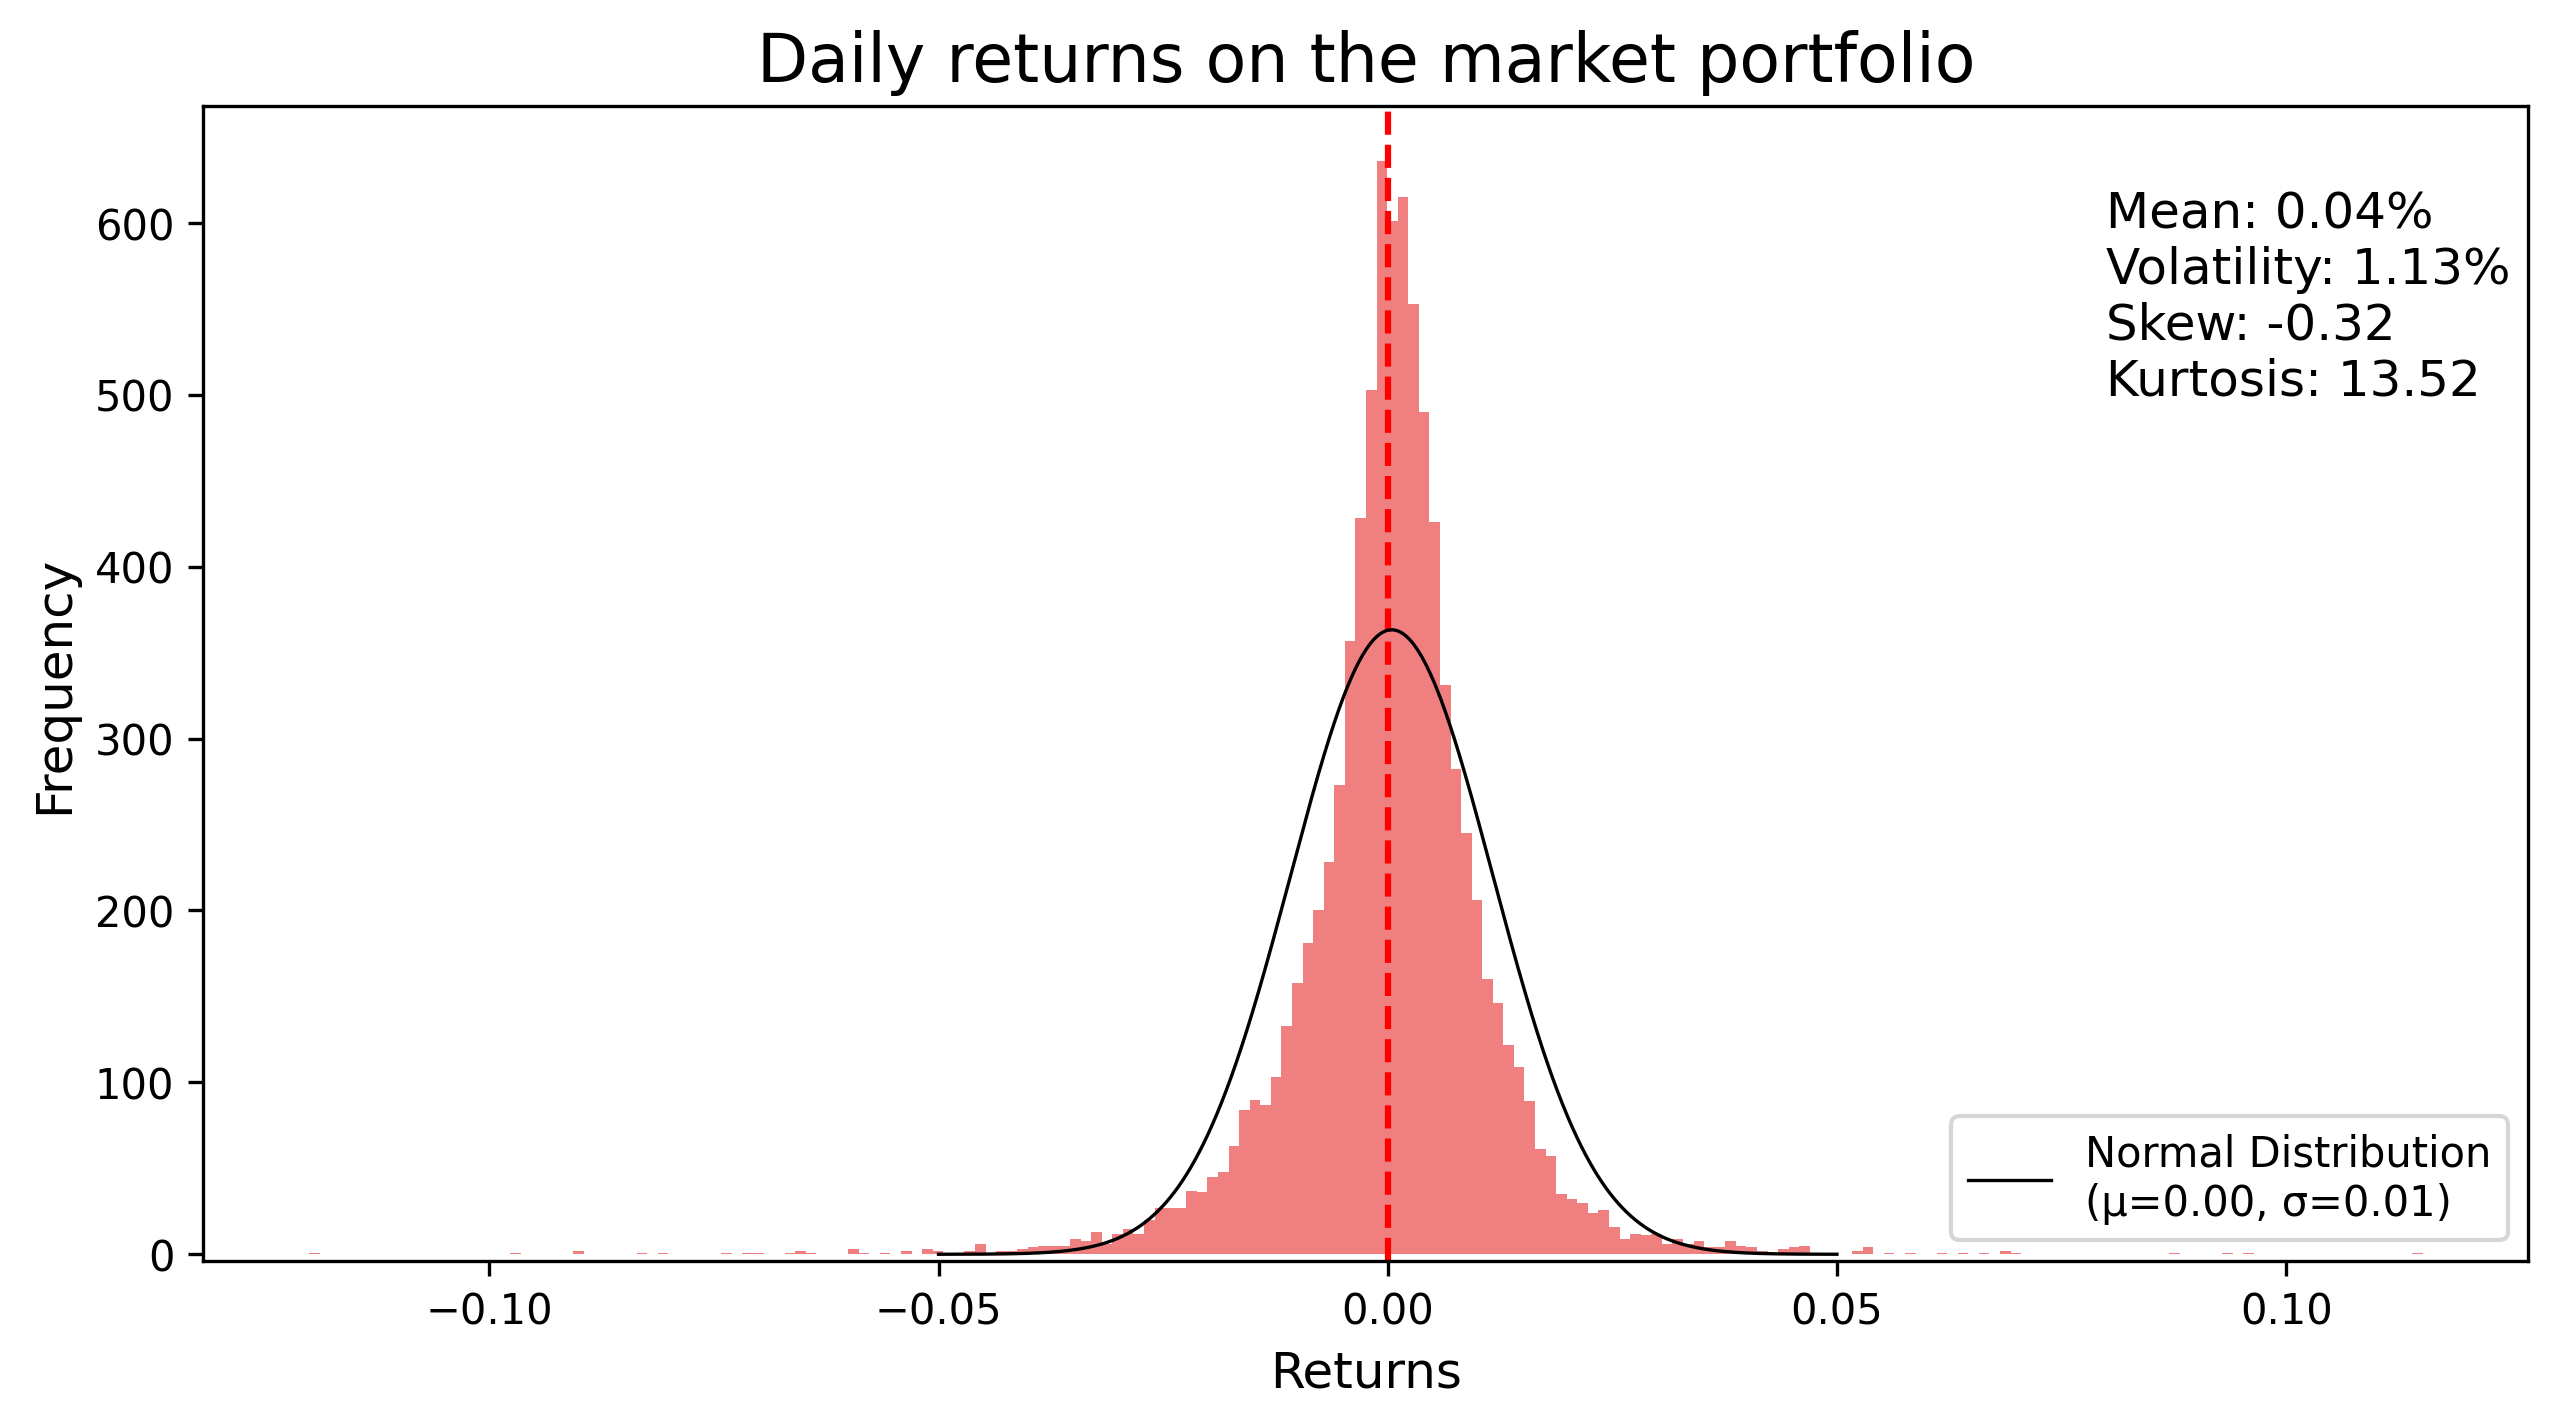
\includegraphics[width=0.75\textwidth]{fig8.png}
    \caption{Distribution of daily returns for the CRSP market portfolio (1988–2022)}
    \label{fig:fig8}
\end{figure}

The data reveal a daily mean return of 0.04\%, a standard deviation of 1.13\%, skewness of –0.32, and kurtosis of approximately 14. A daily return of 0.04\% translates into an average annual return of $0.04 \cdot 250 =  10\%$, while a daily volatility of 1.13\% translates into an annual volatility of $1.13 \cdot \sqrt{250} \approx 17.9\%$.

Unsurprisingly, aggregate returns exhibit negative skewness even though individual stocks often display positive skewness. Idiosyncratic good news (a drug approval, a tech breakthrough) lifts single-firm performance but diversifies away in the index, while broad negative news (macro shocks, liquidity freezes) affects many firms simultaneously, producing a heavier downside tail. Yet, regulations have promoted fairness, orderliness, and efficiency in markets when volatility spikes. In that sense, high volatility markets repeatedly remind investors to “expect the unexpected”.

However, there is one aspect of the unexpected that is notoriously hard to detect. Note that the kurtosis is roughly 14. Kurtosis has a problem that the mean does not have, and the variance has to a much lesser degree: it is biased downwards.

\subsection{Hidden Kurtosis}
Sample kurtosis is supposed to measure the fat tails of a distribution. However, true kurtosis may be much larger than any one sample indicates. 

To test this bias, we simulated $500,000$ market returns using the jump-diffusion model from Section 2, calibrated with the parameter set that \citet{backus2011disasters} link to heavy‐tailed behavior to achieve the high kurtosis and negative skewness associated with market returns (parameters specified in Appendix ~\ref{appendix:code}). We then computed the population kurtosis of this simulated distribution.

To illustrate how sample estimates understate true tail risk, we conducted a Monte Carlo experiment: we took $10,000$ independent random samples of $50$ randomly selected returns each (without replacement) from the simulated population and calculated the sample kurtosis for each draw. \autoref{fig:fig9} shows the distribution of the $10,000$ sample estimates of kurtosis. To obtain an average sample kurtosis of $15$, we need a population kurtosis of over 100.

\begin{figure}[h]
    \centering
    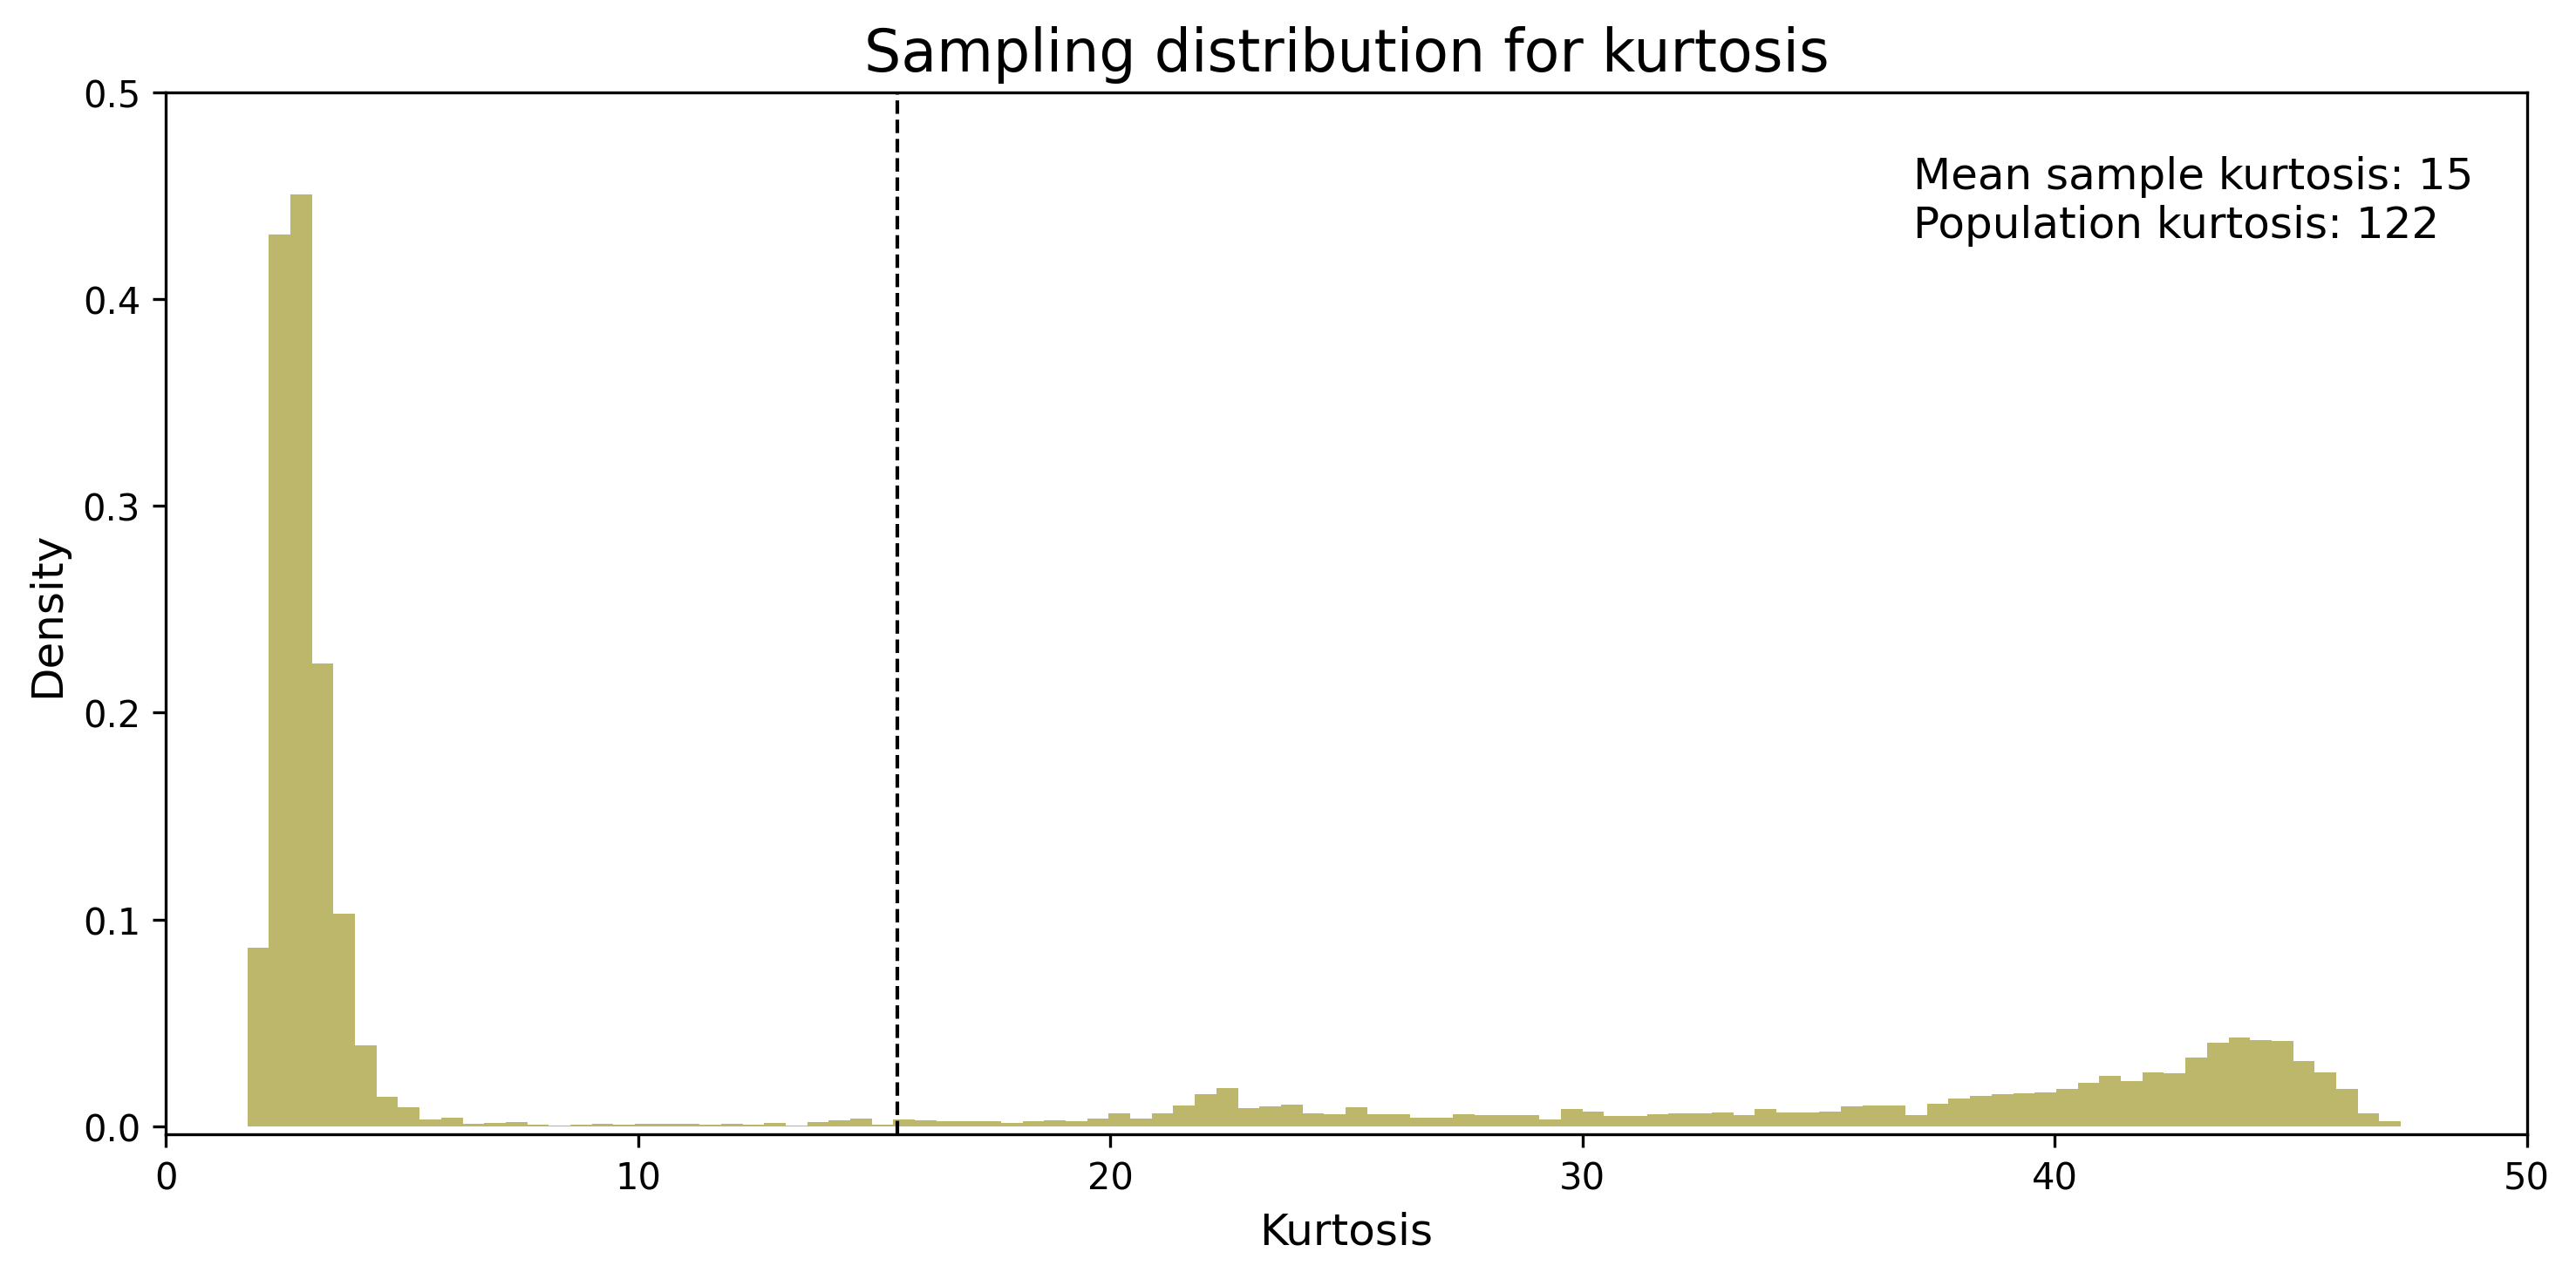
\includegraphics[width=0.75\textwidth]{fig9.png}
    \caption{Distribution of sample kurtosis, where true kurtosis exceeds 100}
    \label{fig:fig9}
\end{figure}

Intuitively, rare events will always catch markets off guard, so it is tempting to lean on statistics such as sample kurtosis for reassurance about tail risk. Yet our simulation shows that even when the true kurtosis exceeds 100, most 50‑day samples report values well below 15. Because small samples almost always understate true kurtosis, they can only tell us that returns are not normal, never that they are safely close to normal. Accurately gauging those fat tails is therefore critical for securities whose pay‑offs are highly sensitive to extreme moves, since underestimating kurtosis means underestimating the probability and cost of rare, severe shocks.